%% START EDUCATION CHAPTER
\chapter{\educationtitle}
\label{chap:education}
\clearpage

With rapid advances in sequencing technologies, the entire field of biology has largely shifted to depend upon the ability to analyze ultra-large datasets. As a result, the ability to perform basic computation has become a necessary prerequisite for successful biological research, yet it is only barely beginning to enter official undergraduate biology curricula as a required topic. Further, these skills are required not only by undergraduate biologists, but by graduate students, post-docs, and even faculty members and professionals, yet these individuals may not have the ability to enroll in undergraduate Computer Science courses. In an attempt to address this gap in education availability, I have dedicated significant effort to develop \glspl{MAIT} for use in \glspl{MOOC} as well as in flipped in-person classrooms.

\section{Introduction}
\subsection{Bioinformatics Education: The New Frontier}
With the introduction of \gls{NGS} technologies, researchers gained the ability to perform large-scale sequencing experiments at extremely high throughput with relatively low costs~\cite{Metzker2010}. Due to the massive sizes of the datasets that are produced in such experiments, basic computational education has become increasingly necessary for successful biological research. While professors at top universities have started introducing bioinformatics courses into undergraduate curricula in recent years~\cite{Compeau2019,Mulder2018,Madlung2018}, access to such courses is typically restricted to students who have the ability to \textit{enroll} in undergraduate courses at these top universities. However, high tuition costs disproportionately prevent low-income and minority students from entering such universities~\cite{Wetzel1998}, leading to disparity in terms of who actually has access to such learning materials. Further, undergraduate students are not the only audience of interest for courses in such topics: graduate students, post-docs, and even faculty and professionals who received formal training in biological and biomedical sciences without any computational coursework are in need of these bioinformatics courses. In addition to difficulties faced by students, due to the rapid growth of the popularity of computational courses~\cite{Camp2017}, instructors of such courses tend to struggle to scale their courses to accommodate large class sizes.

\subsection{The MOOC Revolution}
With the creation of companies like Coursera and edX, university professors started to develop \glspl{MOOC}: tuition-free courses taught over the internet to a large number of students. What started as just a handful of courses, such as \textit{Machine Learning} by Andrew Ng (2012)~\cite{Ng2012}, eventually blew up, and all major universities started releasing \glspl{MOOC} on a wide range of subjects~\cite{Pappano2012}. Much research went into how to design these courses~\cite{Guardia2013,Bruff2013,Breslow2013,Guo2014}. Further, \glspl{MOOC} seemed to attract increased participation by residents of countries in which higher education is extremely rare, far more significant representation of women than in universities, a large proportion of individuals who are either unemployed or seeking to change field of employment, and a considerable number of individuals simply taking courses for interest~\cite{Bayeck2016}. However, their reception was generally mixed: some enjoyed the freedom of filling their education gaps at their own pace~\cite{Milligan2017}, whereas others were pessimistic about their educational value~\cite{Vardi2012}. Many complaints were aimed at the passive learning encompassed in traditional \glspl{MOOC}, in which students simply watch a series of lecture videos and answer simple multiple choice quizzes embedded throughout.

\subsection{From MOOCs to MAITs}
Phillip Compeau and Pavel Pevzner released the first ever bioinformatics \gls{MOOC}, \textit{Bioinformatics Algorithms} (2014)~\cite{Compeau2014}, and with it, a new technology to revolutionize online learning: the \gls{MAIT}, an online text that has integrated quizzes, numerical problems, and even coding challenges to allow the learner to directly interact with the content and to allow the instructor to enable active learning, even in a remote and automated setting~\cite{Compeau2015}. The challenges are adaptive in that they provide the student uniquely-tailored feedback based on the student's specific misconception, and the text itself is adaptive in that the user can take his or her own unique ``learning path.'' For example, a biology student would have the ability to take optional ``detours'' on prerequisite computer science topics such as time complexity, whereas a computer science student would have the ability to take optional ``detours'' on prerequisite biology topics such as the Central Dogma. These carefully-written \glspl{MAIT} were the foundation upon which the \textit{Bioinformatics Algorithms} \glspl{MOOC} were built, and the adaptivity and interactivity was generally well-received by the learners.

\subsection{``Bioinformatics'' Means Nobody Gets Left Behind}
Despite the great success of the \textit{Bioinformatics Algorithms} \glspl{MOOC}, the space of online bioinformatics education was not yet filled: these courses were excellent for students with extensive backgrounds in programming, discrete mathematics, and algorithms, but for all biologists who wanted to transition into the computational aspects of the field, these courses were incomprehensible due to the students' lack of computational background. This motivated my work in bioinformatics education: the development of beginner-friendly \glspl{MAIT} to embed within \glspl{MOOC} as well as to integrate into offline classrooms.

\section{Methods}
\subsection{Teaching Philosophy}
Just like running a traditional offline classroom, developing a \gls{MAIT} requires the implementation of various pedagogical techniques to optimize the learning experience and to enhance student outcomes. As such, the pedagogical design of a \gls{MAIT} is essential to its success. In this section, I discuss the pedagogical techniques I utilize when developing \glspl{MAIT}.

\subsubsection{Bloom's Taxonomy}
Bloom's Taxonomy is a set of three hierarchical models used to classify educational learning objectives into levels of complexity and specificity~\cite{Bloom1956}. The cognitive (i.e., knowledge-based) domain of the taxonomy is a hierarchy containing the following levels: Remember, Understand, Apply, Analyze, Evaluate, and Create (Fig.~\ref{fig:education-bloom-taxonomy})~\cite{Anderson2001}. I follow the guidelines of Bloom's Taxonomy when developing my materials.

\begin{figure}
\centering
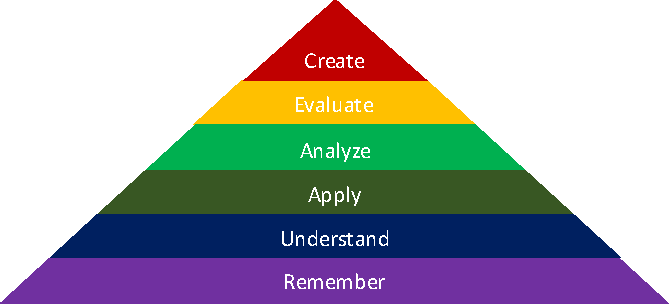
\includegraphics[width=0.65\textwidth]{figs/education-bloom-taxonomy}
\caption[Bloom's Taxonomy]
{Bloom's Taxonomy}
\label{fig:education-bloom-taxonomy}
\end{figure}

\subsubsection{Active Learning}
Within my \glspl{MAIT}, I implement the Active Learning approach: students actively engage with the materials as opposed to simply passively reading or viewing them~\cite{Bonwell1991}. Specifically, I integrate numerous multiple choice, short answer, numerical, and coding challenges that can be solved directly within the text. By undergoing frequent assessment throughout the learning process, students are able to gauge their mastery of concepts \textit{throughout} a given section, and they will be able to correct their misconceptions precisely when they occur (unlike many existing self-paced learning resources, which typically assess student mastery at the \textit{end} of each section).

\subsubsection{Adaptive Learning}
A common misconception is that online education lacks the personalized qualities of an offline course. However, on the contrary, in my \glspl{MAIT}, I demonstrate that my tens of thousands of students are able to receive far more personalized feedback than is possible in an offline class of even tens of students. Specifically, in my \glspl{MAIT}, all challenges (including coding) are automatically graded via carefully-designed \glspl{ITS}, which attempt to provide students uniquely-tailored feedback based on their specific misconceptions (Fig.~\ref{fig:education-code-challenge}).

\begin{figure}
\centering
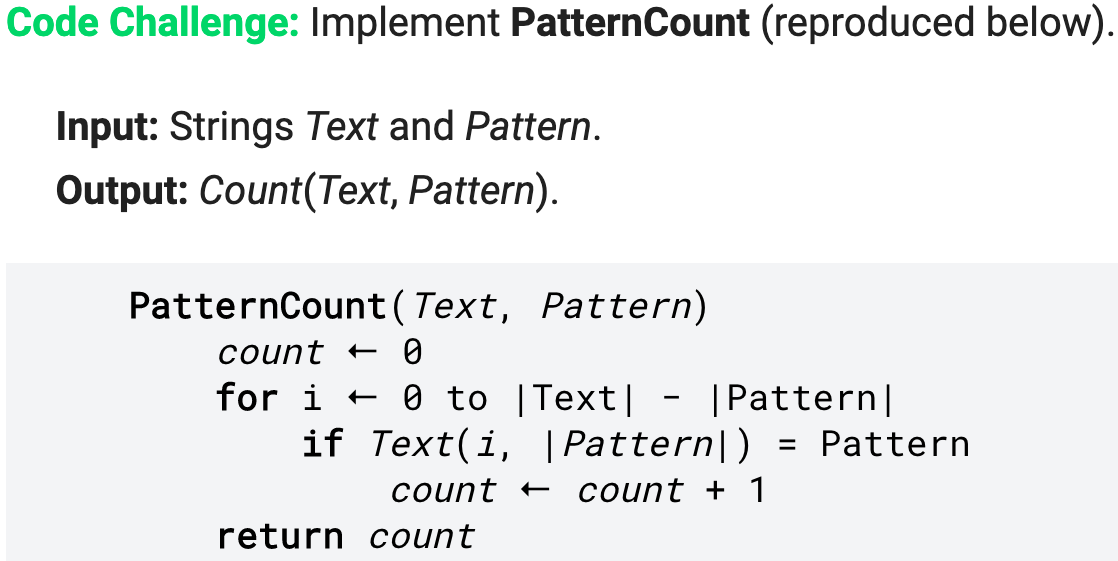
\includegraphics[width=0.85\textwidth]{figs/education-code-challenge-prompt}\\
(a)\\
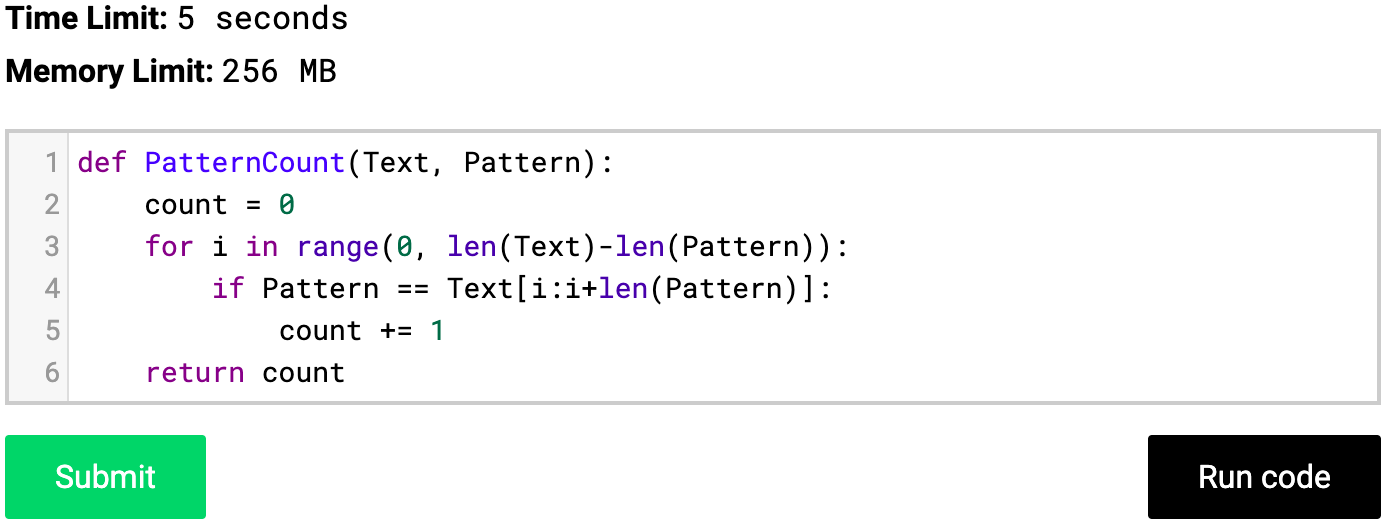
\includegraphics[width=0.85\textwidth]{figs/education-code-challenge-bug}\\
(b)\\~\\
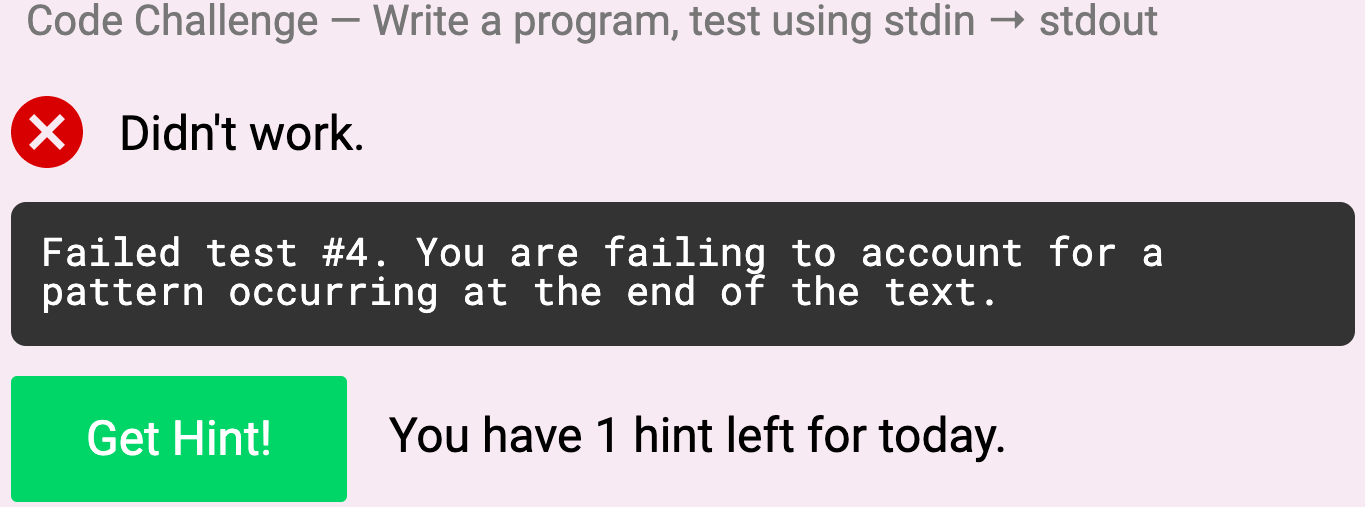
\includegraphics[width=0.85\textwidth]{figs/education-code-challenge-feedback}\\
(c)\\
\caption[Example Code Challenge]
{Example code challenge. (a) Each problem has a clear prompt, and (b) students can solve the problems directly within the text. In this example solution, the student has an off-by-one bug (the student misses the last index), and (c) the carefully-designed \gls{ITS} is able to provide the student personalized feedback.}
\label{fig:education-code-challenge}
\end{figure}

\subsubsection{Inquiry-Based Learning}
In introductory computational courses, the topics that are covered are rarely very interesting when presented out-of-context. When I present new topics in my \glspl{MAIT}, I first motivate them using a real-world problem in the form of a story. By employing Inquiry-Based Learning, an educational strategy in which students perform tasks in a fashion similar to those undertaken by professional scientists in order to construct knowledge~\cite{Pedaste2015}.

\subsubsection{Discovery Learning}
Research into Discovery Learning has showed that, when a student finds the solution to an open-ended problem on their own, the student benefits two-fold: the student typically has a stronger fundamental understanding of the solution, and the student has an improved perception of his or her own abilities to solve problems of this nature~\cite{Bruner1961}. In my \glspl{MAIT}, instead of simply presenting the learning goal to the student, I try to \textit{guide} the students and have them discover the solution on their own.

\subsubsection{Making Learning Fun!}
In my own experiences as a student, I often found it difficult to complete assigned reading assignments and would quickly lose interest during classes. In computational textbooks and learning resources, I often felt as though the learning materials were presented in a manner that was unneededly dry and complex. Instead, I fill my \glspl{MAIT} with stories, jokes, and puns, and I attempt to avoid the use of unnecessarily complex jargon when describing concepts to ensure that students of a wide range of backgrounds are able to follow successfully. I believe the success to learning is in the hands of the \textit{learners}, and it is the responsibility of the teacher as the expert to design the educational journey to be genuinely captivating. Intuitively, it is much easier to teach when students \textit{want} to learn.

\section{Results}
I developed \textit{Analyze Your Genome!} (2017), a \gls{MOOC} designed to teach biologists the best-practice workflows to analyze biological big data~\cite{Moshiri2017b}. However, instead of discussing the specifics of the algorithms behind the analyses, I focused on how to design, execute, and interpret end-to-end bioinformatics experiments. With this approach, students are able to gain the basic proficiency required to perform relevant analyses to complement their traditional biological experiments. The course covered differential gene expression analysis using \gls{RNA}-sequencing data, variant calling using \gls{WGS} vs. \gls{WES} data, rare variant calling and phasing using \gls{WGS} data obtained from a trio (i.e., mother, father, and child), and bacterial genome assembly.

I also developed \textit{Data Structures}, a \gls{MAIT} to accompany the \textit{Advanced Data Structures} course at the University of California, San Diego. Since its initial development, it has been integrated into data structures courses at the University of San Diego and the University of Puerto Rico. In 2017, the \gls{MAIT} was integrated into a \gls{MOOC} on edX: \textit{Data Structures: An Active Learning Approach} (2017)~\cite{Moshiri2017a}. The goal of the \gls{MOOC} was to bridge the gap between introductory programming (which exists in many \glspl{MOOC}) and the \textit{Bioinformatics Algorithms} \glspl{MOOC} by Compeau and Pevzner. After the large success of the \gls{MOOC}, the \gls{MAIT} was adapted to a physical textbook: \textit{Design and Analysis of Data Structures} (2018)~\cite{Moshiri2018c}. In total, \textit{Data Structures} has reached a total of nearly 40,000 learners in less than 3 years of existence, and the learners span a wide range of ages, education levels, and countries (Fig.~\ref{fig:education-learner-demographics}).

\begin{figure}
\centering
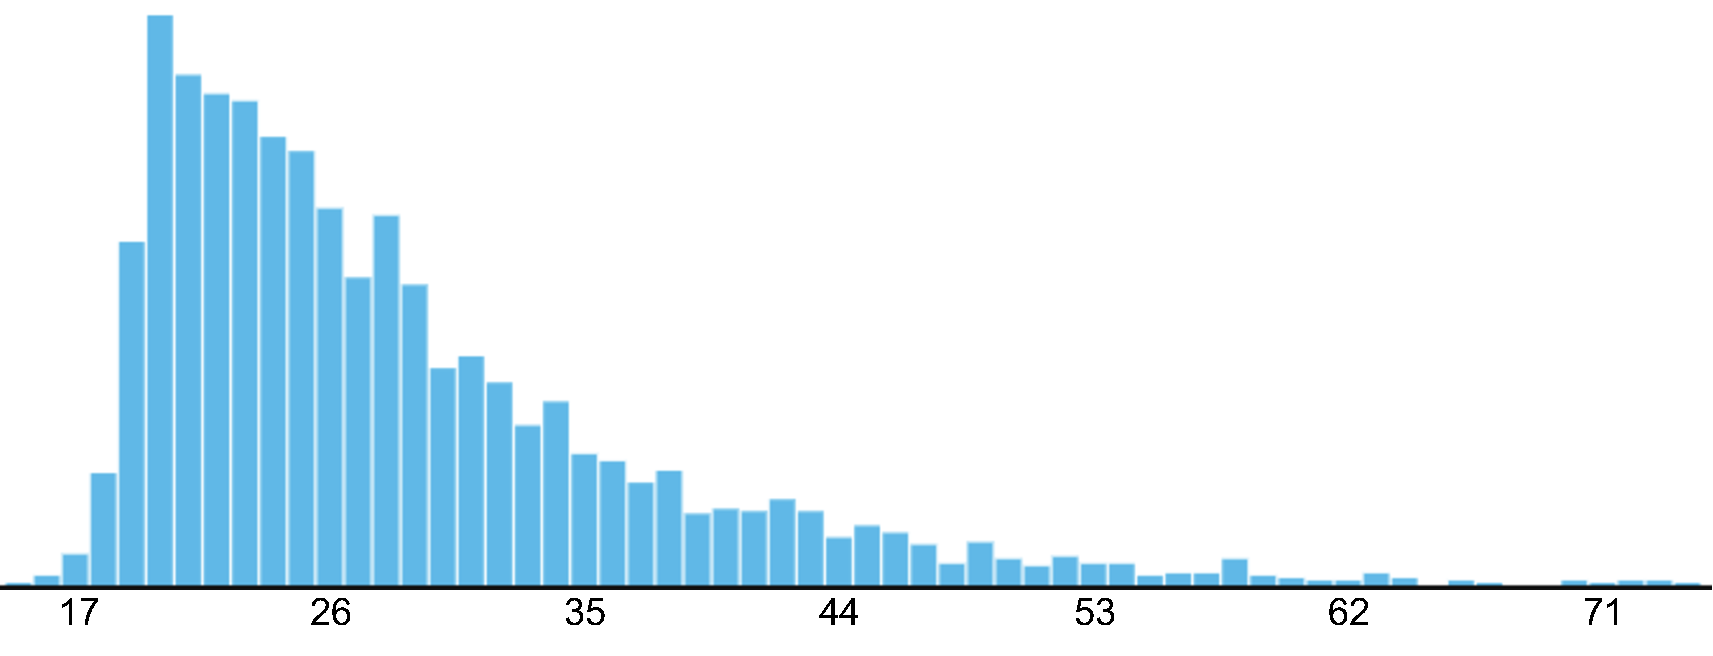
\includegraphics[width=0.85\textwidth]{figs/education-data-structures-learner-ages}\\
(a)\\
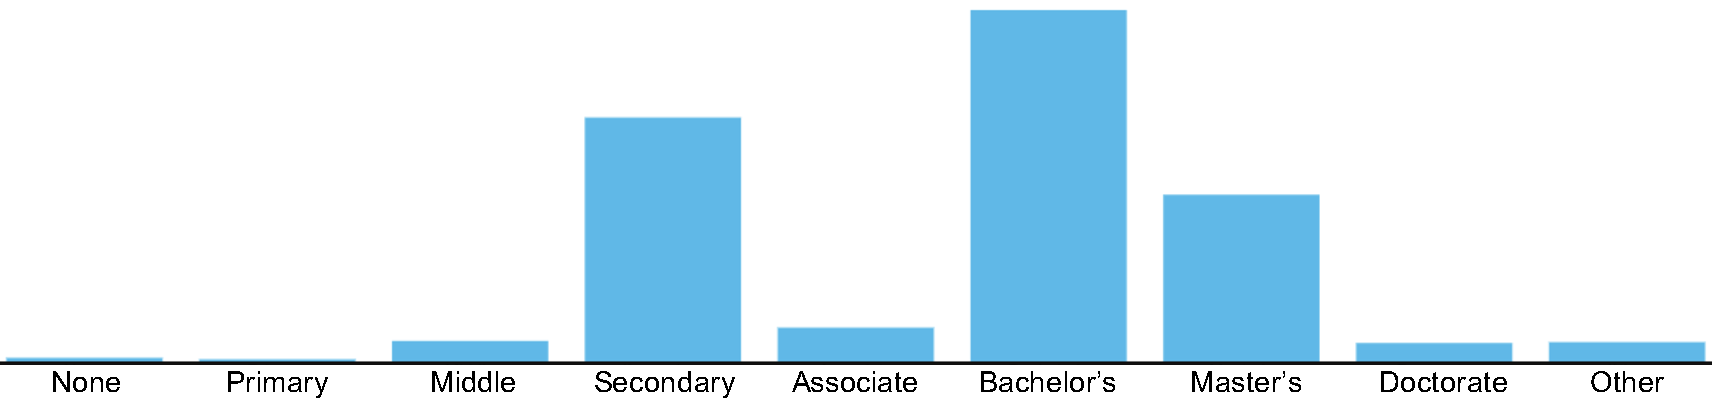
\includegraphics[width=0.85\textwidth]{figs/education-data-structures-learner-education-levels}\\
(b)\\~\\
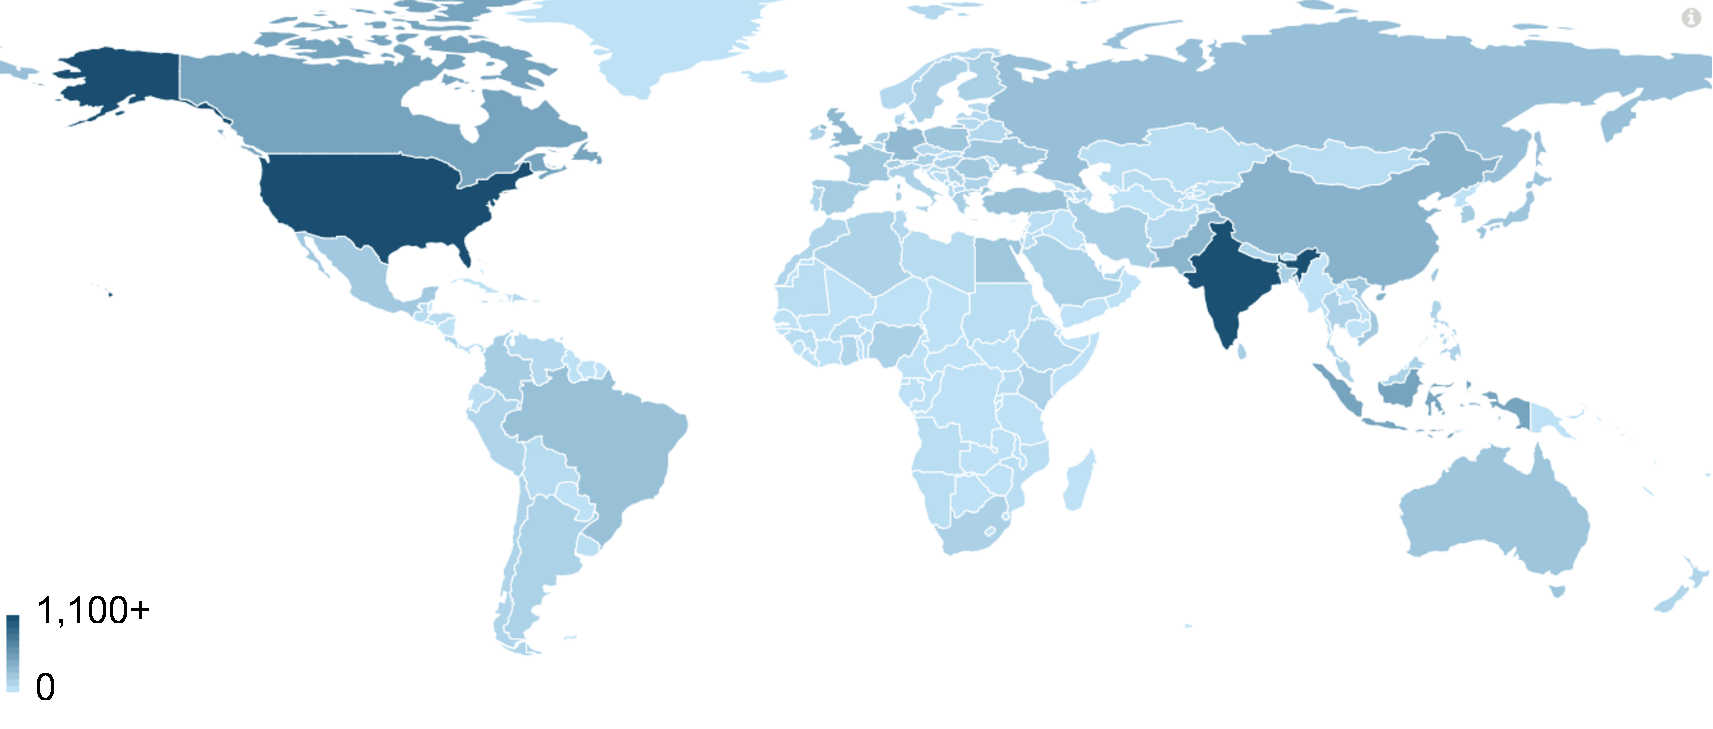
\includegraphics[width=0.85\textwidth]{figs/education-data-structures-learner-country}\\
(c)\\
\caption[Learner Demographics]
{(a) Age distribution, (b) education level distribution, and (c) geographical locations of learners in \textit{Data Structures: An Active Learning Approach}.}
\label{fig:education-learner-demographics}
\end{figure}

\section{Discussion}
Historically, the ability to learn computer science and bioinformatics has been restricted to students in higher education institutions, which can be prohibitive due to financial hardship, time constraints, or other factors. However, due to their self-paced nature, \glspl{MOOC} reduce these barriers to entry, permitting entrance by previously underrepresented demographics. For example, data structures are typically only taught in undergraduate computer science courses, meaning the distribution of students is predominantly within the range of 17 through early 20s, whereas my \gls{MOOC} has reached a far wider range of learners who would otherwise not take such a course (Fig.~\ref{fig:education-learner-demographics}a). Further, MOOCs serve as a unique opportunity for learners who may have formal education in one field but wish to transition fields, such as biologists with Bachelors, Masters, or even Doctorate levels of education who wish to learn introductory computer science (Fig.~\ref{fig:education-learner-demographics}b). Lastly, \glspl{MOOC} are accessible to curious minds across the globe, thus enabling the education of individuals who physically would not be able to attend a top university (Fig.~\ref{fig:education-learner-demographics}c).

Of course, the success of my \gls{MAIT}-based \glspl{MOOC} is largely due to the topics I have chosen, which happen to align well with the automation capabilities of online learning platforms. Specifically, the challenges in my \glspl{MOOC} are largely coding-focused, and it is typically simple to objectively determine the correctness of a student's code. However, topics in other fields (such as the social sciences) may not experience this simple objectivity in assessing correctness, which could lead to difficulties in developing \glspl{ITS} to automate grading and provide personalized feedback. Even within Computer Science and Bioinformatics, coding-focused courses may be prime for this form of presentation, but more theoretical or proof-based courses will certainly not enjoy the same ease of design.

Further, not all students in the same way, and just like any other educational technology or mode of instruction, \glspl{MAIT} may not be the optimal mode of instruction for all students. For example, some students strongly prefer the ability to directly interact with their instructor, and while online education does permit real-time interaction in the form of video meetings, the student may not perceive the interaction to be as meaningful if done remotely. On the other hand, other students who feel lost in large lectures may actually prefer the self-paced and adaptive nature of \glspl{MAIT}, which can provide them a far more personalized learning experience than can an instructor teaching 300+ other students simultaneously.

In short, I believe that, when designed carefully and executed properly, a \gls{MAIT} can be a powerful tool for improving learning and for allowing instructors to reach a massive number of individuals in a highly-scalable fashion. In the future, I will continue to develop high-quality \glspl{MAIT} to address the learning needs of the bioinformatics community.

%% END EDUCATION CHAPTER